\tableofcontents

\newpage

\section{Задание}
По выданному преподавателем варианту разработать программу асинхронного обмена данными с внешним устройством. При помощи программы осуществить ввод или вывод информации, используя в качестве подтверждения данных сигнал (кнопку) готовности ВУ.
\begin{figure}[H]
\centering
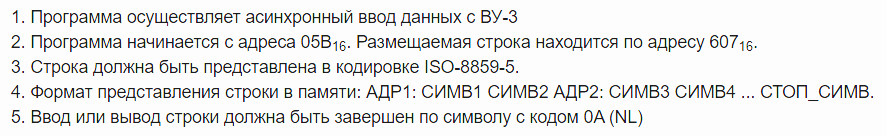
\includegraphics[scale=0.5]{task}
\label{pic:task}
\end{figure}

\section{Текст программы}
\begin{center}
\begin{tabular}{c}
\begin{lstlisting}[basicstyle=\ttfamily]
	ORG	0x05B
ADDR:	WORD	$STRING
NOW:	WORD	0
NL:	WORD	0x0A
GOD:	WORD	0xFF
START:	LD	ADDR
	ST	NOW
NEXT:	CLA
WAIT1:	IN	0x7
	AND	#0x40
	BEQ	WAIT1
	IN	0x6
	SWAB
	ST	(NOW)
	SWAB
	CMP	NL
	BEQ	STOP
	CLA
WAIT2:	IN	0x7
	AND	#0x40
	BEQ	WAIT2
	LD	(NOW)
	IN	0x6
	ST	(NOW)+
	AND	GOD
	CMP	NL
	BNE	NEXT
STOP:	HLT
	ORG	0x607
STRING:	WORD	?
\end{lstlisting}
\end{tabular}
\end{center}

\section{Вводимая строка}
\begin{center}
\begin{tabular}{|c|c|c|c|}
\hline
 & ISO-8859-5 & UTF-8 & UTF-16\\
\hline
О & BE & D0 9E & 041E\\
с & E1 & D1 81 & 0441\\
о & DE & D0 BE & 043E\\
б & D1 & D0 B1 & 0431\\
о & DE & D0 BE & 043E\\
  & 20 & 20 & 0020\\
к & DA & D0 BA & 043A\\
р & E0 & D1 80 & 0440\\
у & E3 & D1 83 & 0443\\
п & DF & D0 BF & 043F\\
н & DD & D0 BD & 043D\\
ы & EB & D1 8B & 044B\\
e & D5 & D0 B5 & 0435\\
  & 20 & 20 & 0020\\
о & DE & D0 BE & 043E\\
с & E1 & D1 81 & 0441\\
о & DE & D0 BE & 043E\\
б & D1 & D0 B1 & 0431\\
и & D8 & D0 B8 & 0438\\
  & 20 & 20 & 0020\\
м & DC & D0 BC & 043C\\
о & DE & D0 BE & 043E\\
г & D3 & D0 B3 & 0433\\
у & E3 & D1 83 & 0443\\
т & E2 & D1 82 & 0442\\
  & 20 & 20 & 0020\\
н & DD & D0 BD & 043D\\
e & D5 & D0 B5 & 0435\\
в & D2 & D0 B2 & 0432\\
о & DE & D0 BE & 043E\\
з & D7 & D0 B7 & 0437\\
б & D1 & D0 B1 & 0431\\
р & E0 & D1 80 & 0440\\
а & D0 & D0 B0 & 0430\\
н & DD & D0 BD & 043D\\
н & DD & D0 BD & 043D\\
о & DE & D0 BE & 043E\\
  & 20 & 20 & 0020\\
з & D7 & D0 B7 & 0437\\
о & DE & D0 BE & 043E\\
х & E5 & D1 85 & 0445\\
а & D0 & D0 B0 & 0430\\
в & D2 & D0 B2 & 0432\\
а & D0 & D0 B0 & 0430\\
т & E2 & D1 82 & 0442\\
ь & EC & D1 8C & 044C\\
  & 20 & 20 & 0020\\
у & E3 & D1 83 & 0443\\
т & E2 & D1 82 & 0442\\
к & DA & D0 BA & 043A\\
у & E3 & D1 83 & 0443\\
, & 2C &    2C & 002C\\
  & 20 & 20 & 0020\\
с & E1 & D1 81 & 0441\\
о & DE & D0 BE & 043E\\
\hline
\end{tabular}
\quad
\begin{tabular}{|c|c|c|c|}
\hline
 & ISO-8859-5 & UTF-8 & UTF-16\\
\hline
б & D1 & D0 B1 & 0431\\
а & D0 & D0 B0 & 0430\\
к & DA & D0 BA & 043A\\
у & E3 & D1 83 & 0443\\
, & 2C &    2C & 002C\\
  & 20 & 20 & 0020\\
л & DB & D0 BB & 043B\\
и & D8 & D0 B8 & 0438\\
ч & E7 & D1 87 & 0447\\
и & D8 & D0 B8 & 0438\\
н & DD & D0 BD & 043D\\
к & DA & D0 BA & 043A\\
у & E3 & D1 83 & 0443\\
  & 20 & 00 20 & 0020\\
ч & E7 & D1 87 & 0447\\
e & D5 & D0 B5 & 0435\\
л & DB & D0 BB & 043B\\
о & DE & D0 BE & 043E\\
в & D2 & D0 B2 & 0432\\
e & D5 & D0 B5 & 0435\\
к & DA & D0 BA & 043A\\
а & D0 & D0 B0 & 0430\\
  & 20 & 20 & 0020\\
и & D8 & D0 B8 & 0438\\
л & DB & D0 BB & 043B\\
и & D8 & D0 B8 & 0438\\
  & 20 & 20 & 0020\\
с & E1 & D1 81 & 0441\\
в & D2 & D0 B2 & 0432\\
о & DE & D0 BE & 043E\\
e & D5 & D0 B5 & 0435\\
г & D3 & D0 B3 & 0433\\
о & DE & D0 BE & 043E\\
  & 20 & 20 & 0020\\
ж & D6 & D0 B6 & 0436\\
e & D5 & D0 B5 & 0435\\
  & 20 & 20 & 0020\\
с & E1 & D1 81 & 0441\\
о & DE & D0 BE & 043E\\
р & E0 & D1 80 & 0440\\
о & DE & D0 BE & 043E\\
д & D4 & D0 B4 & 0434\\
и & D8 & D0 B8 & 0438\\
ч & E7 & D1 87 & 0447\\
а & D0 & D0 B0 & 0430\\
  & 20 & 20 & 0020\\
п & DF & D0 BF & 043F\\
о & DE & D0 BE & 043E\\
х & E5 & D1 85 & 0445\\
и & D8 & D0 B8 & 0438\\
л & DB & D0 BB & 043B\\
e & D5 & D0 B5 & 0435\\
e & D5 & D0 B5 & 0435\\
. & 2E &    2E & 002E\\
\hline
\end{tabular}
\end{center}

\section{Описание программы}
\subsection{Назначение программы}
Программа реализует посимвольный асинхронный ввод с ВУ-3 в кодировке ISO8859-5. В 16-битной ячейке памяти БЭВМ размещается два 8-битных символа, начиная с ячейки 0x607. Цикл ввода продолжается до тех пор, пока не будет введен символ NL (0x0A).

\subsection{Область представления и область допустимых значений данных}
\subsubsection{Область представления данных}
\noindent Ячейки NOW, NL, GOD: 16-разрядные беззнаковые целые числа\\
Ячейки с введенной строкой: 16-разрядные беззнаковые целые числа

\subsubsection{Область допустимых значений данных}
\noindent NL $=const=$ 0x0A\\
GOD $=const=$ 0xFF\\
Длина вводимой строки: 0\ldots1196

\subsection{Расположение в памяти ЭВМ}
\noindent Программа: 05F\ldots075\\
Адрес ячейки первого символа строки: 05B (ADDR)\\
Адрес текущей ячейки записи символов: 05C (NOW)\\
Код символа окончания строки: 05D (NL)\\
Код для отбрасывания первого байта: 05E (GOD)\\
Введенная строка: 607\ldots607 $+$ $\frac{N_{16}+1}{2}$ (без остатка),\\где $N_{16}$ --- длина строки в 16-ричной СС

\subsection{Адреса первой и последней выполняемой команд программы}
\noindent Адрес первой команды программы: 05F\\
Адрес последней команды программы: 075

\section{Таблица трассировки (для первых двух символов)}
\begin{center}
\begin{tabular}{|c|c|c|c|c|c|c|c|c|c|c|c|}
\hline
\multicolumn{2}{|c}{\makecell{\textbf{Выполняемая}\\\textbf{команда}}}
  &\multicolumn{8}{|c|}{\textbf{Содердимое регистров после выполнения команды}}
  &\multicolumn{2}{c|}{\makecell{\textbf{Ячейка, содержимое}\\\textbf{которой изменилось}}}\\
\hline
Адрес & Код & IP & CR & AR & DR & SP & BR & AC & NZVC & Адрес & Новый код\\
\hline
05F & AEFB & 060 & AEFB & 05B & 0607 & 000 & FFFB & 0607 & 0000 & --- & ---\\
\hline
060 & EEFB & 061 & EEFB & 05C & 0607 & 000 & FFFB & 0607 & 0000 & 05C & 0607\\
\hline
061 & 0200 & 062 & 0200 & 061 & 0200 & 000 & 0061 & 0000 & 0100 & --- & ---\\
\hline
062 & 1207 & 063 & 1207 & 062 & 1207 & 000 & 0062 & 0040 & 0100 & --- & ---\\
\hline
063 & 2F40 & 064 & 2F40 & 063 & 0040 & 000 & 0040 & 0040 & 0000 & --- & ---\\
\hline
064 & F0FD & 065 & F0FD & 064 & F0FD & 000 & 0064 & 0040 & 0000 & --- & ---\\
\hline
065 & 1206 & 066 & 1206 & 065 & 1206 & 000 & 0065 & 00BE & 0000 & --- & ---\\
\hline
066 & 0680 & 067 & 0680 & 066 & 0680 & 000 & 0066 & BE00 & 1000 & --- & ---\\
\hline
067 & E8F4 & 068 & E8F4 & 607 & BE00 & 000 & FFF4 & BE00 & 1000 & 607 & BE00\\
\hline
068 & 0680 & 069 & 0680 & 068 & 0680 & 000 & 0068 & 00BE & 0000 & --- & ---\\
\hline
069 & 7EF3 & 06A & 7EF3 & 05D & 000A & 000 & FFF3 & 00BE & 0001 & --- & ---\\
\hline
06A & F00A & 06B & F00A & 06A & F00A & 000 & 006A & 00BE & 0001 & --- & ---\\
\hline
06B & 0200 & 06C & 0200 & 06B & 0200 & 000 & 006B & 0000 & 0101 & --- & ---\\
\hline
06C & 1207 & 06D & 1207 & 06C & 1207 & 000 & 006C & 0040 & 0101 & --- & ---\\
\hline
06D & 2F40 & 06E & 2F40 & 06D & 0040 & 000 & 0040 & 0040 & 0001 & --- & ---\\
\hline
06E & F0FD & 06F & F0FD & 06E & F0FD & 000 & 006E & 0040 & 0001 & --- & ---\\
\hline
06F & A8EC & 070 & A8EC & 607 & BE00 & 000 & FFEC & BE00 & 1001 & --- & ---\\
\hline
070 & 1206 & 071 & 1206 & 070 & 1206 & 000 & 0070 & BEE1 & 1001 & --- & ---\\
\hline
071 & EAEA & 072 & EAEA & 607 & BEE1 & 000 & FFEA & BEE1 & 1001 & 05C & 0608\\
\hline
--- & --- & --- & --- & --- & --- & --- & --- & --- & --- & 607 & BEE1\\
\hline
072 & 2EEB & 073 & 2EEB & 05E & 00FF & 000 & FFEB & 00E1 & 0001 & --- & ---\\
\hline
073 & 7EE9 & 074 & 7EE9 & 05D & 000A & 000 & FFE9 & 00E1 & 0001 & --- & ---\\
\hline
074 & F1EC & 061 & F1EC & 071 & F1EC & 000 & FFEC & 00E1 & 0001 & --- & ---\\
\hline
061 & 0200 & 062 & 0200 & 061 & 0200 & 000 & 0061 & 0000 & 0101 & --- & ---\\
\hline
062 & 1207 & 063 & 1207 & 062 & 1207 & 000 & 0062 & 0040 & 0101 & --- & ---\\
\hline
063 & 2F40 & 064 & 2F40 & 063 & 0040 & 000 & 0040 & 0040 & 0001 & --- & ---\\
\hline
064 & F0FD & 065 & F0FD & 064 & F0FD & 000 & 0064 & 0040 & 0001 & --- & ---\\
\hline
065 & 1206 & 066 & 1206 & 065 & 1206 & 000 & 0065 & 000A & 0001 & --- & ---\\
\hline
066 & 0680 & 067 & 0680 & 066 & 0680 & 000 & 0066 & 0A00 & 0001 & --- & ---\\
\hline
067 & E8F4 & 068 & E8F4 & 608 & 0A00 & 000 & FFF4 & 0A00 & 0001 & 608 & 0A00\\
\hline
068 & 0680 & 069 & 0680 & 068 & 0680 & 000 & 0068 & 000A & 0001 & --- & ---\\
\hline
069 & 7EF3 & 06A & 7EF3 & 05D & 000A & 000 & FFF3 & 000A & 0101 & --- & ---\\
\hline
06A & F00A & 075 & F00A & 06A & F00A & 000 & 000A & 000A & 0101 & --- & ---\\
\hline
075 & 0100 & 076 & 0100 & 075 & 0100 & 000 & 0075 & 000A & 0101 & --- & ---\\
\hline
\end{tabular}
\end{center}

\section{Вывод}
В ходе выполнения данной лабораторной работы я познакомился с взаимодействием внешних устройств с БЭВМ, работой ввода-вывода и новыми для меня командами - IN, OUT. Также мною был изучен новый способ ввода программ - с использованием ассемблера. Эти знания пригодятся мне для дальнейшей работы с БЭВМ и понимания работы современных ЭВМ.
